\documentclass[Review,times,sageh]{sagej}

\usepackage{moreverb,url,natbib, multirow, tabularx}
\usepackage[colorlinks,bookmarksopen,bookmarksnumbered,citecolor=red,urlcolor=red]{hyperref}


% Pandoc citation processing

\usepackage{cleveref}
\providecommand{\tightlist}{\setlength{\itemsep}{0pt}\setlength{\parskip}{0pt}}



\begin{document}

\title{Analytic choices for analyzing multidimensional behavior: Many analysts test hypotheses about human speech}

\runninghead{Many analysts, one speech data set}

\author{Stefano Coretta*\affilnum{1}, Timo Roettger\affilnum{2}, Joseph V. Casillas\affilnum{3}}

\affiliation{\affilnum{1}{Institute of Phonetics and Speech Processing, Ludwig-Maximilian University Munich, Germany.}\\\affilnum{2}{Department of Applied Things, University B, City B, Country B}\\\affilnum{3}{Very Important Stuff Committee, Institute C, City C, Country C}}

\corrauth{Stefano Coretta}

\email{\href{mailto:s.coretta@lmu.de}{\nolinkurl{s.coretta@lmu.de}}}

\begin{abstract}
TBA
\end{abstract}

\keywords{crowdsourcing science, data analysis, scientific transparency, speech, acoustic analysis}

\maketitle

\hypertarget{introduction}{%
\section{Introduction}\label{introduction}}

In order to effectively accumulate knowledge, science needs to (i) produce data that can be replicated using the original methods and (ii) arrive at robust conclusions substantiated by the data.
In recent coordinated efforts to replicate published findings, scientific disciplines have uncovered surprisingly low success rates \citep[e.g.,][]{open2015estimating, camerer2018evaluating} leading to what is now referred to as the \emph{replication crisis}.
Beyond the difficulties of replicating scientific findings, a growing body of evidence suggests that the theoretical conclusions drawn from data are often variable even when researchers have access to reliable data.
The latter situation has been referred to as the \emph{inference crisis} \citep{rotello2015more, starns2019assessing} and is, among other things, rooted in the inherent flexibility of data analysis \citep[often referred to as researcher degrees of freedom:][]{simmons2011false, gelman2014statistical}.
Data analysis involves many different steps, such as inspecting, organizing, transforming, and modeling the data, to name a few.
Along the way, different methodological and analytic choices need to be made, all of which may influence the final interpretation of the data.
These researcher degrees of freedom are both a blessing and a curse.

They are a blessing because they afford us the opportunity to look at nature from different angles, which, in turn, allows us to make important discoveries and generate new hypothesis \citep[e.g.,][]{box1976science, tukey1977exploratory, de2014thought}.
They are a curse because idiosyncratic choices can lead to categorically different interpretations, which eventually find their way into the publication record where they are taken for granted \citep{simmons2011false}.
Recent projects have shown that the variability between different data analysts is vast and can lead independent researchers to draw different conclusions from the same data set \citep[e.g.,][]{silberzahn2018many, starns2019assessing, botvinik2020variability}.
These studies, however, might still underestimate the extent to which analysts vary because data analysis is not merely restricted to statistical inference.
Human behavior is complex and offers many ways to be translated into numbers.
This is particularly true for fields that draw conclusions about human behavior and cognition from multidimensional data like audio or video data.
In fields working on human speech production, for example, researchers need to make numerous decisions about what to measure and how to measure it.
This is not trivial, given the temporal extension of the acoustic signal and its complex structural composition.
Not only can decisions about measuring the signal influence downstream decisions about statistical modeling, but statistical results or modeling issues can also lead researchers to go back and revise earlier decisions about the measuring process itself.

In this article, we investigate the variability in analytic choices when many analyst teams analyze the same speech production data set, a process that involves both decisions regarding the operationalization of a complex signal and decisions regarding the statistical analysis.
Specifically, we discuss the impact of analytic decision making on research results obtained by N teams who had access to the same set of acoustic recordings in order to answer the same research question.

\hypertarget{researcher-degrees-of-freedom}{%
\subsection{Researcher degrees of freedom}\label{researcher-degrees-of-freedom}}

Data analysis comes with many decisions, like how to measure a given phenomenon or behavior, which data to submit to statistical modeling and which to exclude in the final analysis, or what inferential decision-making procedure to apply.
This can be problematic because humans show cognitive biases that can lead to erroneous inferences.
Humans filter the world in irrational ways \citep[e.g.,][]{tversky1974judgment}, seeing coherent patterns in randomness \citep{brugger2001}, convincing themselves of the validity of prior expectations \citep[``I knew it'',][]{nickerson1998confirmation}, and perceiving events as being plausible in hindsight \citep[``I knew it all along'',][]{fischhoff1975hindsight}.
In conjunction with an academic incentive system that rewards certain discovery processes more than others \citep{sterling1959publication, koole2012rewarding}, we often find ourselves exploring many possible analytic pipelines, but only reporting a selected few.

This issue is particularly amplified in fields in which the raw data lend themselves to many possible ways of being measured \citep{roettger2019researcher}.
Combined with a wide variety of methodological and theoretical traditions as well as varying levels of statistical training across subfields, the inherent flexibility of data analysis might lead to a vast plurality of analytic approaches that can lead to different scientific conclusions.
Analytic flexibility has been widely discussed from a conceptual point of view \citep{simmons2011false, wagenmakers2012agenda, nosek2014method} and in regard to its application in individual scientific fields \citep[e.g.][]{wicherts2016, charles2019, roettger2019researcher}.
This notwithstanding, there are still many unknowns regarding the extent of analytic plurality in practice.

Consequently, it is likely that a good part of published papers present overconfident interpretations of data and statistical results based on idiosyncratic analytic strategies \citep[e.g.,][]{simmons2011false, gelman2014statistical}.
These interpretations, and the conclusions that derive from them, are thus associated with an unknown degree of uncertainty (dependent on the strength of evidence provided) and with an unknown degree of generalisability (dependent on the chosen analysis).
Moreover, the same data could lead to very different conclusions depending on the analytic path taken by the researcher.
However, instead of being critically evaluated, scientific results often remain unchallenged in the publication record.
Despite recent efforts to improve transparency and reproducibility \citep[e.g.][]{miguel2014promoting, klein2018practical} and the advent of freely available and accessible infrastructures, such as those provided by the Open Science Framework (osf.io), critical re-analyses of published analytic strategies are still uncommon because data sharing remains rare \citep{wicherts2006poor}.

\hypertarget{crowdsourcing-alternative-analyses}{%
\subsection{Crowdsourcing alternative analyses}\label{crowdsourcing-alternative-analyses}}

Recent collaborative attempts have started to shed light on how different analysts tackle the same data set and have revealed a large amount of variability.
In a collaborative effort, \citet{silberzahn2018many} let twenty-nine independent analysis teams address the same research hypothesis.
Analytic approaches and consequently the results varied widely between teams.
Sixty-nine percent of the teams found support for the hypothesis, and 31\% did not.
Out of the 29 analytic strategies, there were 21 unique combinations of covariates.
Importantly, the observed variability was neither predicted by the team's preconceptions about the phenomenon under investigation nor by peer ratings of the quality of their analyses.
The authors results suggest that analytic plurality may be an inevitable byproduct of the scientific process and not necessarily driven by different levels of expertise nor bias.

Several other recent studies corroborated this analytic flexibility across different disciplines.
\citet{dutilh2019} ad \citet{starns2019assessing} investigated analysts' choices when inferring theoretical constructs based on the same data set using computational models.
Both studies revealed vastly different modeling strategies, even though scientific conclusions were similar across analysis teams \citetext{\citealp[see also][ on analytic flexibility in ecology]{Parker2020}; \citealp[and][ on neuroimaging data]{botvinik-nezer2020}}.
\citet{bastiaansen2020} crowdsourced clinical recommendations based on analyses of an individual patient.
Results suggests that analysts differed substantially regarding decisions related to both the statistical analysis of the data and the theoretical rationale behind interpreting the statistical results.

While these studies attested a large degree of analytic flexibility with possibly impactful consequences, they only investigated analytic decisions related to inferential statistics or the architecture of computational models.
In these studies the data sets were fixed and neither data collection nor measurement could be changed.
However, in many fields the primary raw data are complex signals that need to be operationalized relative to a theoretically motivated research question.
This is especially true in the social sciences, where the phenomenon under investigation corresponds to both observable and unobservable human behavior.

Decisions about how to measure a theoretical construct related to human behavior or its underlying cognitive processes might interact with downstream decisions about statistical modeling and vice versa.
For instance, \citet{flake2020} discuss the cascading impact that different practices can have on psychometric research.
The authors highlight, among others, the following degrees of freedom in the choice and development of measures: definition of the theoretical construct, justification of the selected measure, description of the measure and of how it maps onto the construct, response coding and related transformations, and post-hoc modifications to the chosen measure.
Taken together, these aspects alone exponentially increase the combinations of possible analytic choices, and hence flexibility in research outcomes.

In those disciplines concerned with communication, human behavior sometimes corresponds to multidimensional visual or acoustic signals.
The complex nature of this data multiplies the number of possible analytic approaches, thus further increasing analytic flexibility.
The present study looks at experimentally elicited speech production data in order to understand how this flexibility manifests itself in a scenario where several procedures are involved in the operationalization and measuring of complex signals.

\hypertarget{s:operspeech}{%
\subsection{Operationalizing speech}\label{s:operspeech}}

Research on speech is at the heart of the cognitive sciences, informing psychological models of language, categorization, and memory, guiding methods for diagnosis and therapy of speech disorders, and facilitating advancement in automatic speech recognition and speech synthesis.
One major challenge in the speech sciences is the mapping between communicative intentions (the unobserved behavior) and their physical manifestation (the observed behavior).

Speech is a complex signal that is characterized by structurally different acoustic landmarks distributed throughout different temporal domains.
Thus, choosing how to measure a phenomenon of interest is an important analytic decision.
Take for example the following sentence in (1).

\vspace{1em}

\begin{enumerate}
\def\labelenumi{(\arabic{enumi})}
\tightlist
\item
  ``I can't bear another meeting on Zoom.''
  \vspace{1em}
\end{enumerate}

Depending on the speaker's intention, this sentence can be said in different ways.
For instance, if the speaker is exhausted by all their meetings, they might acoustically highlight the word \emph{another} or \emph{meeting} to contrast it with other, more pleasant activities.
If, on the other hand, the speaker is just tired of video conferences, as opposed to say face-to-face meetings, they might acoustically highlight the word \emph{Zoom}.

If we decide to compare the speech signal associated with these two intentions, how can we quantify the difference between them?
In other words, given their physical manifestation (speech), what do we measure and how do we measure it?
Because of the continuous and transient nature of speech, identifying speech parameters and temporal domains within which to measure those parameters becomes a non-trivial task.
Utterances stretch over several thousand milliseconds and contain different levels of linguistically relevant units such as phrases, words, syllables, and individual sounds.
The researcher is thus confronted with a considerable number of parameters and combinations thereof to choose from.

Speech categories are inherently multidimensional and dynamic: they consist of clusters of parameters that are modulated over time.
The acoustic parameters of one category are usually asynchronous, i.e.~they appear at different time points in the unfolding signal, and overlap with parameters of other categories \citep[e.g.][]{jongman2000acoustic, lisker1986voicing, summerfield1981articulatory, winter2014spoken}.
A classical example is the distinction between voiced and voiceless stops in English (i.e.~/b/ and /p/ in \emph{bear} vs \emph{pear}).
This lexical contrast is manifested by many acoustic features which can differ depending on several factors, such as position of the consonant in the word and surrounding sounds \citep{lisker1977rapid}.
Furthermore, correlates of the contrast can even be found away from the consonant, in temporally distant speech units.
For example, the initial /l/ of the English words \emph{led} and \emph{let} is affected by the voicing of the final consonant (/t, d/) \citep{hawkins2004influence}.

The multiplicity of phonetic cues grows exponentially if we look at larger temporal domains as is the case for suprasegmental aspects of speech.
For example, studies investigating acoustic correlates of word stress (e.g.~the difference between \emph{ínsight} and \emph{incíte}) have been using a wide variety of measurements, including temporal characteristics (duration of certain segments or sub-segmental intervals), spectral characteristics (intensity, formants, and spectral tilt), and measurements related to fundamental frequency (f0) \citep[e.g.,][]{gordon2017acoustic}.
Moving on to the expression of higher-level functions, like information structure and discourse pragmatics, relevant acoustic cues can be distributed throughout even larger domains, such as phrases and whole utterances \citep[e.g.,][]{ladd2008intonational}.
Differences in position, shape, and alignment of pitch modulations over multiple locations within a sentence are correlated with differences in discourse functions (e.g.~Niebuhr et al., 2011).
The latter can also be expressed by global vs local pitch modulations \citep{heuven2002}, as well as acoustic information within the temporal or spectral domain \citep[e.g.,][]{van2005speech}.
Extra-linguistic information, like the speaker's intentions, levels of emotional arousal or social identity, are also conveyed by broad-domain parameters, such as voice quality, rhythm, and pitch \citep{foulkes2006, ogden2004, white2009}.

In short, when testing hypotheses on speech production data, researchers are faced with many choices and possibilities.
The larger the functional domain (e.g.~segments vs words vs utterances), the higher the number of conceivable operationalizations.
For example, several decisions have to be made when comparing the two realizations of the sentence in (1), one of which is intended to signal emphasis on \emph{another} and one of which emphasizes \emph{Zoom}.

\vspace{1em}

(2a) I can't bear \emph{ANOTHER} meeting on Zoom.

(2b) I can't bear another meeting on \emph{ZOOM}.

\vspace{1em}

Do we compare only the word \emph{another} in (2a) and (2b), or also the word \emph{Zoom}?
Do we measure utterance-wide acoustic profiles, whole words, or just the stressed syllables?
Do we average across the chosen time domain or do we measure a specific point in time?
Do we measure fundamental frequency, intensity, or something else?



\begin{figure}
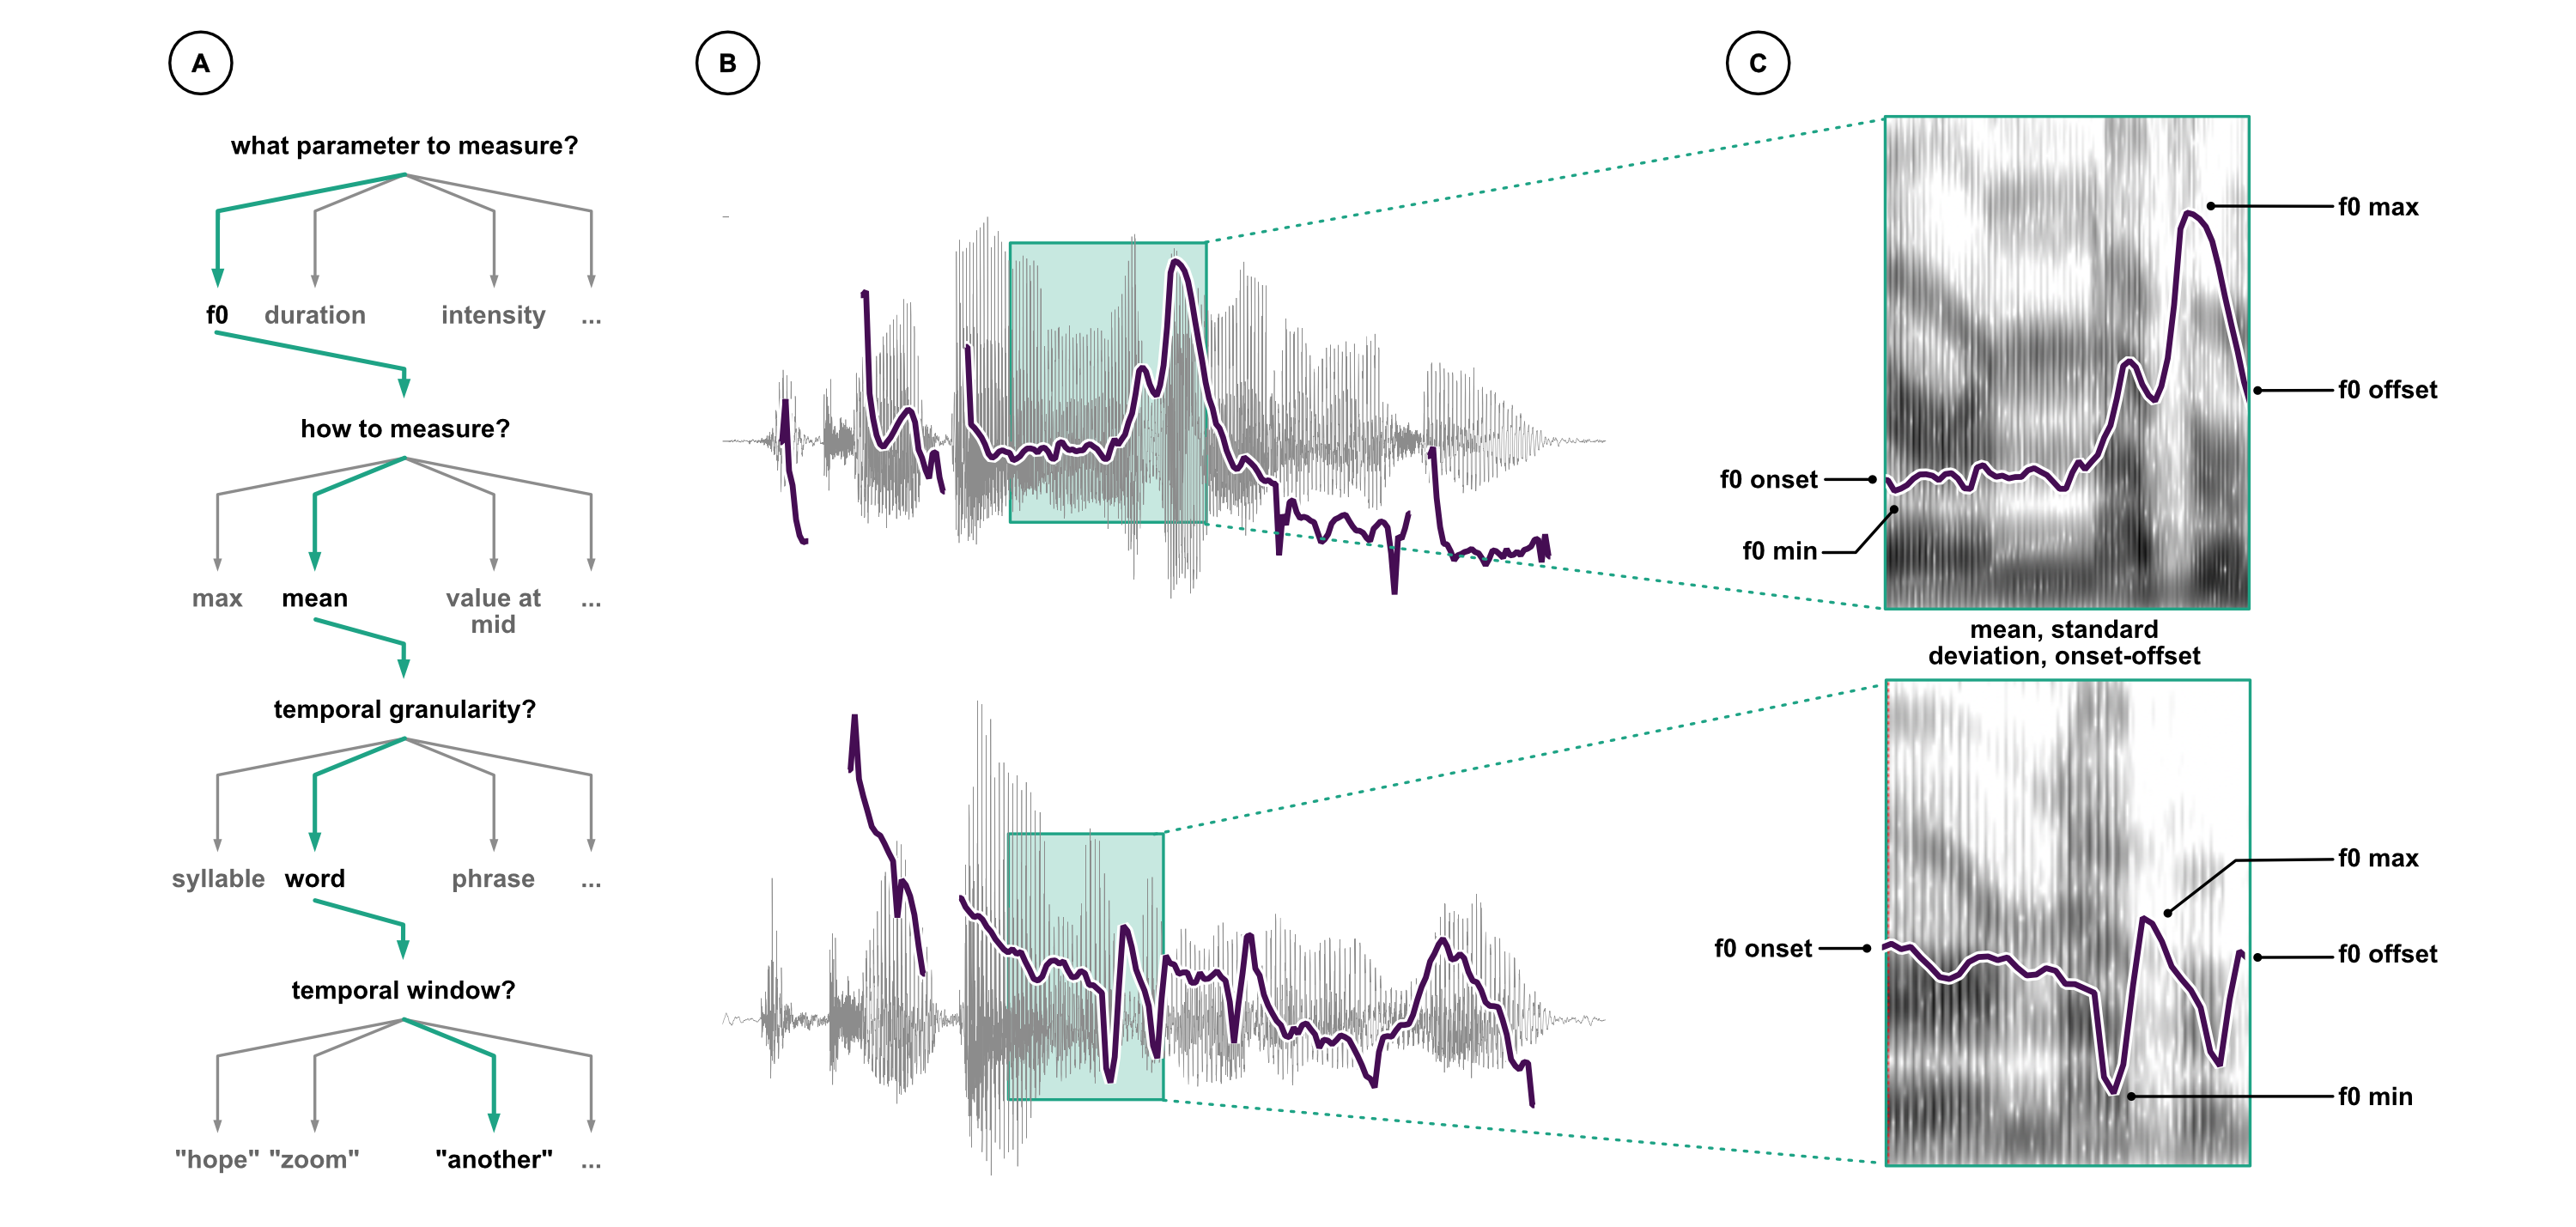
\includegraphics[width=1\linewidth]{/Users/ste/repos/many_analyses/figs/ForkingPaths} \caption{Illustration of the analytic flexibility associated with acoustic analyses. (A) An example of multiple possible and justifiable decisions when comparing two utterances; (B) Waveform and fundamental frequency (f0) track of the utterances \emph{I can't bear ANOTHER meeting on Zoom} and \emph{I can't bear another meeting on ZOOM}. The green boxes mark the word \emph{another} in both sentences; (C) Spectrogram and f0 track of the word \emph{another}, exemplifying possible operationalizations of differences in f0.}\label{fig:forkingPaths}
\end{figure}

When looking at phrase-level temporal domains, the number of alternative analytic pipelines substantially increases.
Figure \ref{fig:forkingPaths}A shows a typical example of a decision tree which speech researcher are often confronted with.
Each of the four analytic decisions in the example have different possible options.
Here only one particular path has been taken, and a different one would likely produce quite different results.
Once we have decided to compare fundamental frequency of the word \emph{another} across the two utterances, there are still many choices to be made, all of which need to be justified.
As Figures \ref{fig:forkingPaths}B-C illustrate, we could measure f0 at specific points in time like the onset of the temporal window, the offset, or the midpoint.
We could also measure the value or time of the minimum or maximum f0 value.
We could summarize f0 across the entire window and extract the mean, median or standard deviation of f0, all of which have been used to analyze speech data in previous work \citep[see][]{gordon2017acoustic}.
But the journey in the garden of analytic paths goes on.
Other important operationalization steps could involve filtering the audio signal, smoothing the extracted f0 track, removing values that substantially deviate from surrounding values or expectations, either manually or automatically, and so on.

These decisions are intended to be made prior to any statistical analysis, but are at times revised a posteriori (i.e.~after data collection and/or preliminary analyses) in light of unforeseen or surprising outcomes.
These myriads of possible decisions are multiplied by those researcher degrees of freedom related to statistical analysis \citep[e.g.][]{wicherts2016}.
In sum, speech data is made of complex physical signals that generates an as-of-yet unappreciated amount of analytic flexibility in the choice of measures and operationalizations.
The present paper probes this garden of forking paths in the analysis of speech.
To assess the variability in data analysis pipelines across independent researchers, we provided analytic teams with an experimentally elicited speech production data set.
The data set derives from the unpublished research project \emph{Prosodic encoding of redundant referring expressions}, which set out to investigate whether speakers acoustically modify utterances to signal unexpected referring expressions.
In the following section we introduce the research question and the experimental procedure of said project, and we describe the resulting data set as used in the current study.

\hypertarget{s:dataset}{%
\subsection{The data set: The acoustic properties of atypical modifiers}\label{s:dataset}}

Referring is one of the most basic and prevalent uses of language and one of the most widely researched areas in language science.
It is an open question how speakers choose a referring expression when they want to refer to a specific entity like a banana.
The context within which an entity occurs (i.e., with other non-fruits, other fruits, or other bananas) plays a large part in determining the choice of referring expressions.
Generally, speakers aim to be as informative as possible to uniquely establish reference to the intended object, but they are also resource-efficient in that they avoid redundancy \citep{grice1975logic}.
Thus one would expect the use of a modifier, for example, only if it is necessary for disambiguation.
For instance, one might use the adjective \emph{yellow} to describe a banana in a situation in which there is a yellow and a less ripe green banana available, but not when there is only one banana to begin with.

Despite the coherent idea that speakers are both rational and efficient, there is much evidence that speakers are often over-informative.
Speakers use referring expressions that are more specific than strictly necessary for the unambiguous identification of the intended referent \citep{sedivy2003pragmatic, westerbeek2015stored, rubio2016redundant}, which has been argued to facilitate object identification and making communication between speakers and listeners more efficient \citep{arts2011overspecification, paraboni2007generating, rubio2016redundant}.
Recent findings suggest that the utility of a referring expression depends on how good it is for a listener (compared to other referring expressions) to identify a target object.
For example, \citet{degen2020redundancy} showed that modifiers that are less typical for a given referent (e.g.~a blue banana) are more likely to be used in an over-informative scenario (e.g.~when there is just one banana).
This account, however, has mainly focused on content selection \citep{gatt2013we}, i.e.~whether a certain referential expression is chosen or not, while not taking into consideration the indexical potential of speech.

Even when morphosyntactically identical expressions are involved, speakers can modulate utterances via suprasegmental acoustic properties like temporal and spectral modifications \citep[e.g.,][]{ladd2008intonational}.
Most prominently, languages use intonation to signal discourse relationships between referents, among other functions.
Intonation marks discourse-relevant referents for being new or given information, to guide the listeners' interpretation of incoming messages.
Beyond structuring information relative to the discourse, a few studies suggested that speakers might use intonation to signal atypical lexical combinations \citep[e.g.][]{dimitrova2008prosodic, dimitrova2009did}.
Referential expressions such as \emph{blue banana} were produced with greater prosodic prominence than more typical referents such as \emph{yellow banana}.
These results are in line with the idea of resource-efficient, rational language users who modulate their speech in order to facilitate listeners' comprehension.
However, the above studies are based on a rather small sample size (10 participants) and on potentially anti-conservative statistical analyses, leaving reason to doubt the generalisability of the studies' conclusions.

To further illuminate the question of whether speakers modify speech to signal atypical referents, and overcome some of the limitations of previous work, thirty native German speakers were recorded in a production study while interacting with a confederate (one of the experimenters) in a referential game.
The participants had to verbally instruct the confederate to select a specified target object out of four objects presented on a screen.
The subject and confederate were seated at the opposite sides of a table, each facing one of two mirrored computer screens.
The participant and the experimenter could not see each other nor each others' screens.
Figure \ref{fig:procedural} shows the experimental procedure time-line.
After a familiarization phase, the subject first saw four colored objects in the top left, top right, bottom left, and bottom right corners of the screen.
One of the objects served as the target, another as the competitor, and the remaining two objects served as distractors.
Objects were referred to using noun phrases consisting of an adjective modifier denoting color and a modified object (e.g.~\emph{Gelbe Zitrone} `yellow lemon', \emph{Rote Gurke} `red cucumber', \emph{Rote Socken} `red socks').



\begin{figure}
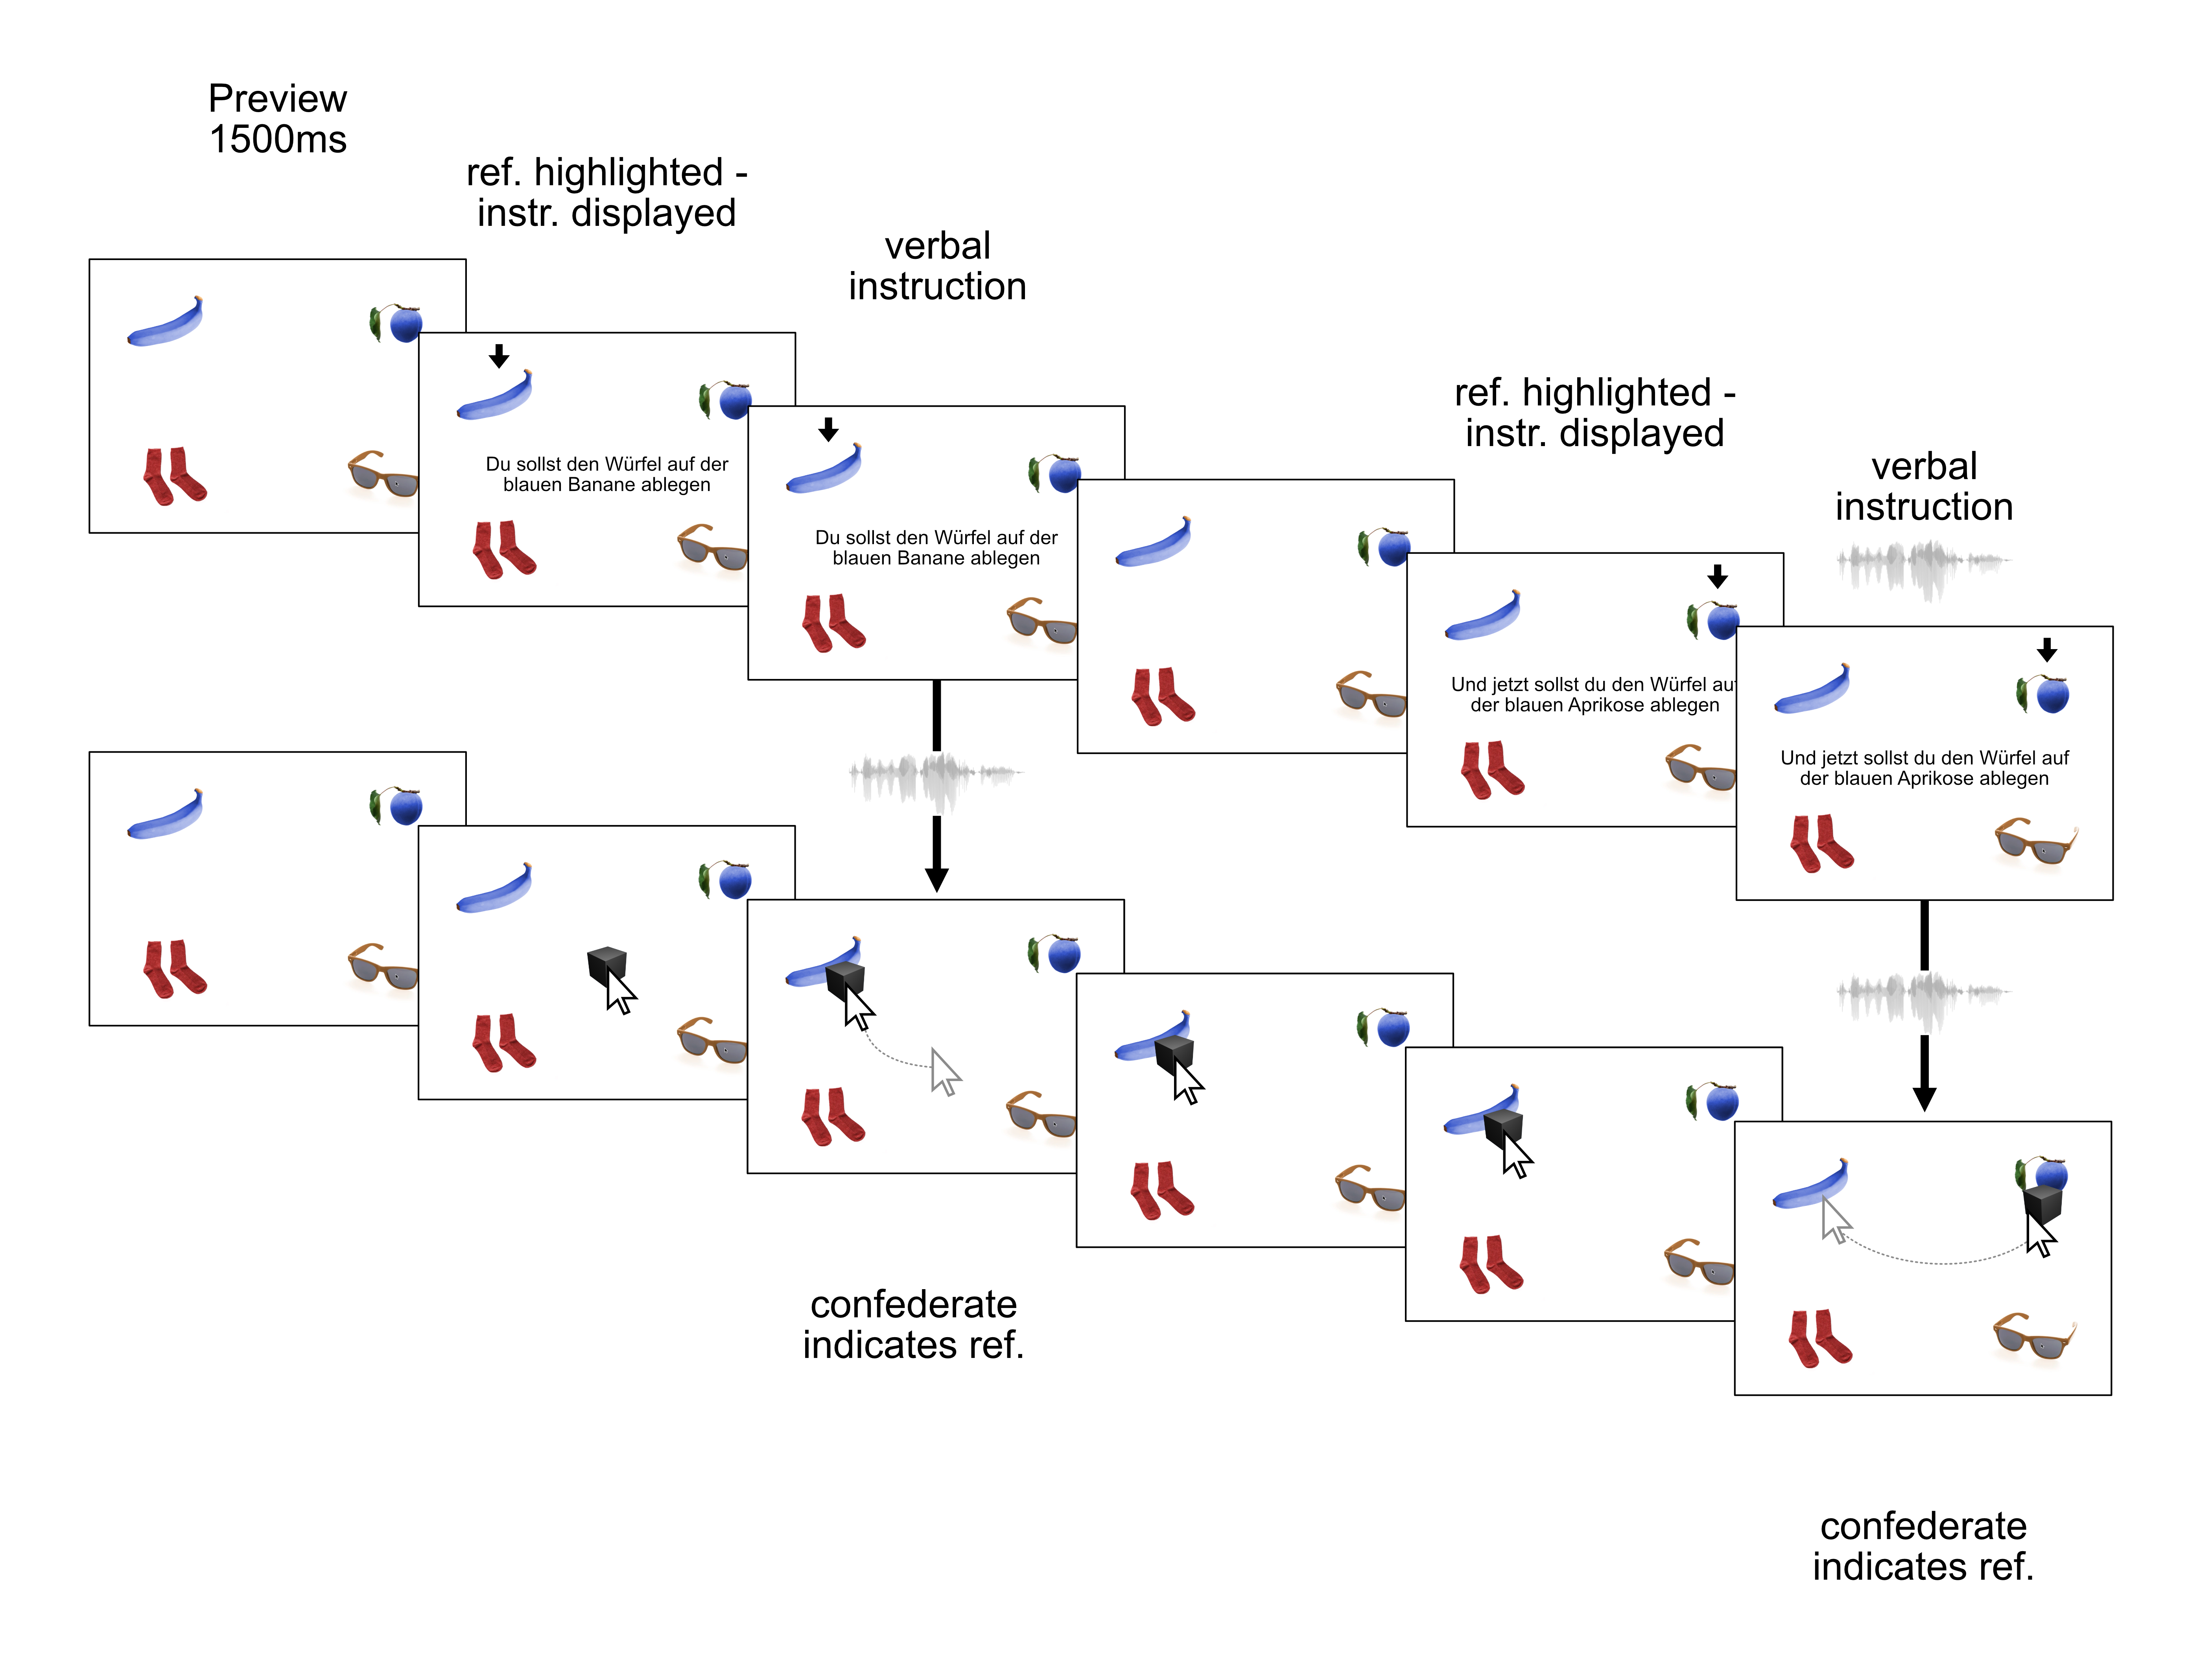
\includegraphics[width=1\linewidth]{/Users/ste/repos/many_analyses/figs/procedure_plot} \caption{Experimental procedure. The upper row illustrates the trial sequence for the speaker (participant) and the lower row illustrates the trial sequence for the confederate. After a preview of 1500ms the speaker sees an arrow indicating one of the referent (b). Reading the orthographic instructions out loud, the speaker gives the confederate verbal instructions onto which referent they should drag the cube (c). The confederate, in turn, drags the black cube onto the target referent (d). Both the arrow and the orthographic instruction disappear from the speaker's screen and a new referent is indicated by an arrow on the same display alongside a new orthographic instruction (e). The speaker gives the confederate verbal instructions (f) which the confederate follows by dragging the cube onto the next referent (g).}\label{fig:procedural}
\end{figure}

In the center of the screen, a black cube was displayed, which could be moved by the experimenter.
The participant would read a sentence prompt out loud (\emph{Du sollst den Würfel auf der COLOR OBJECT ablegen} `You have to put the cube on top of the COLOR OBJECT') to instruct the experimenter to drag the cube on top of one of the four depicted objects (the \emph{competitor}) using the mouse.
After the experimenter had moved the cube as instructed, the subject would read another sentence prompt (\emph{Und jetzt sollst du den Würfel auf der COLOR OBJECT ablegen} `And now, you have to put the cube on top of the COLOR OBJECT') instructing the experimenter to move the cube on top of a different object (the \emph{target}).
The second utterance in the trial was the critical trial for analysis.

The two sentence prompts were used to create a focus contrast between the competitor and the target object.
If the competitor and target objects differ but their color did not (e.g.~\emph{yellow banana} vs \emph{yellow tomato}), the narrow focus is on the noun (the Noun Focus condition, NF).
If the objects are the same but differ in color (e.g.~\emph{yellow banana} vs \emph{blue banana}), the narrow focus is on the color adjective (the Adjective Focus condition, AF).
If both the color and the object differ (e.g.~\emph{yellow banana} vs \emph{blue tomato}), the narrow focus is on the whole noun phrase (the Adjective/Noun Focus condition, ANF).
The NF condition constituted the experimentally relevant condition, while the AF and ANF conditions acted as fillers.
Crucially, the color-object combinations in the Noun Focus (NF) condition were manipulated with respect to their typicality.
The combinations were either typical (e.g.~\emph{orange mandarin}), medium typical (e.g.~\emph{green tomato}), or atypical (e.g.~\emph{yellow cherry}), as established by a norming study that was conducted prior to the production experiment just described.\footnote{A detailed description of the norming and production studies from the \emph{Prosodic encoding of redundant referring expressions} project, which was given to the analysts with the data set, can be found in \texttt{methods\_norm\_prod.pdf} at (temporary link) \url{https://osf.io/5agn9/?view_only=3429acfd8eae4f0aafe2e17ad5b0983f}}
Each subject produced 15 critical trials (NF condition).
Each trial was repeated twice, yielding a total of 30 trials per participant and a grand-total of 900 (\(15 \times 2 \times 30\) participants) spoken utterances.

For the present study, N analysis teams were given access to the entire data set generated by the production study and were instructed to answer the following research question: \emph{Do speakers acoustically modify utterances to signal atypical word combinations in referring expressions?}
\ldots{}

\hypertarget{methods}{%
\section{Methods}\label{methods}}

As outlined in Section \protect\hyperlink{s:operspeech}{Operationalizing speech}, researchers are faced with a large amount of analytic choices when analyzing a multidimensional signal such as speech.
Analysts must identify and operationalize relevant measurements, as well as the temporal domain(s) from which these measurements are to be taken, and then possibly transform said measurements before submitting them to statistical models, which must be chosen alongside inferential criteria.
The complexity of speech data constitutes the ideal testing ground to assess the upper bound of analytic flexibility that social science might face across disciplines.
We will employ a meta-analytic approach to assess (i) the variability of the reported effects, and (ii) how analytic and researcher-related predictors affect the final results.

In this study, we are follow the data collection procedure proposed by \citet{Parker2020}.
The project involves the following five phases:

\begin{enumerate}
\def\labelenumi{\arabic{enumi}.}
\tightlist
\item
  \textsc{Recruitment}: We will recruit independent groups of researchers to analyze the data.
\item
  \textsc{Team Analysis}: We will give researchers access to the speech corpus and let them analyze the data as they see fit.
\item
  \textsc{Review}: We will ask reviewers to generate peer-review ratings of the analyses based on methods (not results).
\item
  \textsc{Meta-analysis}: We will evaluate variability among the different analyses and how different predictors affect the outcomes.
\item
  \textsc{Write-up}: Lastly, we will collaboratively produce the final manuscript.
\end{enumerate}

We estimate that this process, from the time of an in-principle acceptance of this Stage 1 Registered Report to the end of Phase 5, will take nine months.
The factor most likely to delay our time-line is the rate of completion of the original set of analyses by independent analysis teams.

\hypertarget{phase-1-recruitment-of-analysts-and-initial-survey}{%
\subsection{Phase 1: Recruitment of analysts and initial survey}\label{phase-1-recruitment-of-analysts-and-initial-survey}}

An online landing page will provide a general description of the project, including a short pre-recorded slide-show that summarizes the data set and research question (\url{https://many-speech-analyses.github.io}).
The project will be advertised via social media, using mailing lists for linguistic and psychological societies, and via word of mouth.\footnote{Terms in small caps in this and later sections are included with their definition in the glossary at the end of the paper for the reader's convenience.}
The target population comprises active speech science researchers with a graduate/doctoral degree (or currently studying for a graduate/doctoral degree) in relevant disciplines.
Researchers can choose to work independently or in a small team.
For the sake of simplicity, we will refer both to a single researcher and teams as \textsc{analysis teams}.
Recruitment for this project will commence upon receiving in-principle acceptance.
As outlined above, our aim is to assess the variability of the reported effects and how these are affected by a set of predictors, rather than the meta-analytic estimate of the investigated effect \emph{per se}.
Given the scarcity of previous meta-analytic studies that directly investigate researcher's degrees of freedom, as reviewed in the introduction, we are not able to establish a properly-grounded minimal sample size.
Thus, we aim to recruit as many teams as possible, within the resource and time limits of the project.

We will simultaneously recruit volunteers to peer-review the analyses conducted by the analysis teams through the same channels.
Our goal is to recruit a similar number of peer-reviewers and analysts, and to ask each peer-reviewer to review a minimum of four analyses.
If we are unable to recruit at least half the number of reviewers as analysis teams, we will ask analysts to serve also as reviewers (after they have completed their analyses).

All analysts and reviewers will share co-authorship on this manuscript and will participate in the collaborative process of producing the final manuscript.
Informed consent will be obtained as part of the intake form.

\hypertarget{phase-2-primary-data-analyses}{%
\subsection{Phase 2: Primary Data Analyses}\label{phase-2-primary-data-analyses}}

The analysis teams will register for participation and each of the analysts individually will answer a demographic and expertise questionnaire (\texttt{intake\_form.pdf}).
PDF versions of all the questionnaires used in this study are available at LINK\footnote{Temporary link: \url{https://osf.io/h6z8w/?view_only=3457f2b01a5f4435b3d917eb7b5134e8}.}.
The questionnaire collects information on the analysts current position and self-estimated breadth and level of statistical expertise and acoustic analysis skills.
We will then request that they answer the question: \emph{Do speakers acoustically modify utterances to signal atypical word combinations?}
To do so, they will be given the data generated by the experiment described in Section \protect\hyperlink{s:dataset}{The data set}.
The data will include the audio recordings with corresponding time-aligned transcriptions in the form of Praat TextGrid files (LINK\footnote{Temporary link: \url{https://osf.io/5agn9/?view_only=3429acfd8eae4f0aafe2e17ad5b0983f}}).

Once their analysis is complete, they will answer a structured questionnaire (\texttt{analytic\_quest.pdf}), providing information about their analysis technique, an explanation of their analytic choices, their quantitative results, and a statement describing their conclusions.
They will also upload their analysis files (including the additionally derived data and text files that were used to extract and pre-process the acoustic data), their analysis code (if applicable), and a detailed journal-ready statistical methods section.

\hypertarget{phase-3-peer-review-of-analyses}{%
\subsection{Phase 3: Peer Review of Analyses}\label{phase-3-peer-review-of-analyses}}

At a minimum, each analysis will be evaluated by four different reviewers, and each peer-reviewer will be randomly assigned to analyses from at least four analysis teams (the exact number will depend on the number of analysis teams and peer-reviewers recruited).
Each peer-reviewer will register and answer a demographic and expertise questionnaire identical to that asked of the analysts.
Reviewers will evaluate the methods of each of their assigned analyses one at a time in a sequence determined by the initiating authors.
The sequences will be systematically assigned so that, if possible, each analysis is allocated to each position in the sequence for at least one reviewer.

The process for a single reviewer will be as follows.
First, the reviewer will receive a description of the methods of a single analysis.
This will include the narrative methods section, the analysis team's answers to the questionnaire regarding their methods, including analysis code and the data set.
The reviewer will then be asked in an online questionnaire (\texttt{peer\_review\_quest.pdf}) to rate both the acoustic and the statistical analyses and to provide an overall rating, using a scale of 0-100, respectively.
To help reviewers calibrate their rating, they will be given the following guidelines:

\begin{itemize}
\item
  \begin{enumerate}
  \def\labelenumi{\arabic{enumi}.}
  \setcounter{enumi}{99}
  \tightlist
  \item
    A perfect analysis with no conceivable improvements from the reviewer.
  \end{enumerate}
\item
  \begin{enumerate}
  \def\labelenumi{\arabic{enumi}.}
  \setcounter{enumi}{74}
  \tightlist
  \item
    An imperfect analysis but the needed changes are unlikely to dramatically alter final interpretation.
  \end{enumerate}
\item
  \begin{enumerate}
  \def\labelenumi{\arabic{enumi}.}
  \setcounter{enumi}{49}
  \tightlist
  \item
    A flawed analysis likely to produce either an unreliable estimate of the relationship or an over-precise estimate of uncertainty.
  \end{enumerate}
\item
  \begin{enumerate}
  \def\labelenumi{\arabic{enumi}.}
  \setcounter{enumi}{24}
  \tightlist
  \item
    A flawed analysis likely to produce an unreliable estimate of the relationship and an over-precise estimate of uncertainty.
  \end{enumerate}
\item
  \begin{enumerate}
  \def\labelenumi{\arabic{enumi}.}
  \setcounter{enumi}{-1}
  \tightlist
  \item
    A dangerously misleading analysis, certain to produce both an estimate that is wrong and a substantially over-precise estimate of uncertainty that places undue confidence in the incorrect estimate.
  \end{enumerate}
\end{itemize}

The reviewers will also be given the option to include further comments in a text box for each of the three ratings.

After submitting the review, a methods section from a second analysis will then be made available to the reviewer.
This same sequence will be followed until all analyses allocated to a given reviewer have been provided and reviewed.
After providing the final review, the reviewer will be simultaneously presented with all four (or more) methods sections that the reviewer has just completed reviewing, the option to revise their original ratings, and a text box to provide an explanation.

\hypertarget{phase-4-evaluating-variation}{%
\subsection{Phase 4: Evaluating variation}\label{phase-4-evaluating-variation}}

The initiating authors (SC, JC, TR) will conduct the analyses outlined in this section.

\hypertarget{descriptive-statistics}{%
\subsubsection{Descriptive statistics}\label{descriptive-statistics}}

We will calculate summary statistics describing variation among analyses, including (a) the nature and number of acoustic measures (e.g.~f0 or duration), (b) the operationalization and the temporal domain of measurement (e.g.~mean of an interval or value at specified point in time), (c) the nature and number of model parameters for both fixed and random effects (if applicable), (d) the nature and reasoning behind inferential assessments (e.g.~dichotomous decision based on \emph{p}-values, ordinal decision based on a Bayes factor), as well as the (e) mean, (f) standard deviation and (g) range of the standardizes effect sizes (see the next section for the standardization procedure).

\hypertarget{s:meta-est}{%
\subsubsection{Meta-analytic estimation}\label{s:meta-est}}

We will investigate the variability in \textsc{reported effect sizes} using Bayesian meta-analytic techniques.
As the measure of variability, we will take the meta-analytic \textsc{group-level standard deviation} (\(\sigma_{\alpha_{\text{t}}}\), see below), where the groups are the analysis teams.

Based on the common practices currently in place within the field, we anticipate that researchers will use multi-level/hierarchical/mixed-effects regression models, thus common measurements of effect size, such as Cohen's \(d\), may be inappropriate.
Since the variables used by the analysis teams might substantially differ in their measurement scales (e.g, Hertz for frequency vs milliseconds for duration), we will standardize all reported effects by refitting each \textsc{reported model} with centered and scaled continuous variables (\emph{z}-scores, i.e.~the observed values subtracted from the mean divided by the standard deviation) and sum-coded factor variables.
Factor-level ordering for each categorical variable will mirror that of the original analyses.
Each \textsc{standardized model} will be fitted as a Bayesian regression model with Stan \citep{stan2021}, RStan \citep{stan2020a}, and brms \citep{burkner2017} in R \citep{R-base}.
For those reported models that were originally fitted within a frequentist approach, uniform distributions will be used as the priors of all parameters (with the restriction that only positive numbers will be included for scale parameters), making the standardized models in fact equivalent to the reported frequentist models.
If a team has fitted Bayesian models, the same priors as reported by the team will be used in fitting the respective standardized model.

The coefficients of the critical predictors (i.e.~critical according to the analysis teams' self-reported inferential criteria) obtained from the standardized models will be used as the \textsc{standardized effect size} (\(\eta_i\)) of each reported model.
If multiple predictors within a single analysis have been reported as critical, each will be included in the meta-analytic model (described in details in the next paragraph).
Moreover, to account for the differing degree of uncertainty around each standardized effect size, we will use the standard deviation of each standardized effect size as the \textsc{standardized standard error} (\(\text{se}_i\)).
This will enable us to fit a so-called ``measurement-error'' model, in which both the standardized effect sizes and their respective standard errors are entered in the meta-analytic model.
As a desired consequence, effect sizes with a greater standard error will be weighted less than those with a smaller standard error in the meta-analytic calculations.

After having obtained the standardized effect sizes \(\eta_i\) with related standard errors \(\text{se}_i\), for each critical predictor of the individual reported model, we will fit a \textsc{Bayesian random-effects meta-analysis} using a multilevel (intercept-only) regression model.
The outcome variable will be the set of standardized effect sizes \(\eta_i\).
The likelihood of \(\eta_i\) is assumed to correspond to a normal distribution \citep{knight2000}.
The analysis teams will be entered as a group-level effect (i.e., \texttt{(1\ \textbar{}\ team)}, called \emph{random effect} in the frequentist literature).
The standard errors \(\text{se}_i\) will be included as the standard deviation of \(\eta_i\) to fit a measurement-error model, as discussed above.
We will use regularizing weakly-informative priors for the intercept \(\alpha\) (\(Normal(0, 1)\)) and for the group-level standard deviation \(\sigma_{\alpha_{\text{t}}}\) (\(HalfCauchy(0, 1)\)).
We will fit this model with 4 chains of Hamiltonian Monte-Carlo sampling for the estimation of the joint posterior distribution, using the No U-Turn Sampler (NUTS) as implemented in Stan \citep{stan2021}, and 4000 iterations (2000 for warm-up) per chain, distributed across 4 processing cores.
In case of divergent transitions, we will increase \texttt{adapt\_delta}, \texttt{tree\_depth}, and the number of iterations in this order until we obtain a model fit with no divergent transitions.
The analysis will be conducted in R \citep{R-base} and fit using Stan \citep{stan2021}, RStan \citep{stan2020a}, and brms \citep{burkner2017}.
The code used to run the model can be found at \url{https://many-speech-analyses.github.io/suppl/simulations.html}.

The posterior distribution of the population-level intercept \(\alpha\) will allow us to estimate the range of probable values of the standardized effect size \(\hat{\eta}\).
The posterior distribution will further allow us to investigate the effect of a set of analytic and researcher-related predictors, detailed in the next section.
Crucially, the posterior distribution of the \href{.smallcaps}{group-level standard deviation} \(\sigma_{\alpha_{\text{t}}}\) (i.e.~the standard deviation of the group-level effect of team) will allow us to quantify the degree of variation between the teams' analyses on a standardized scale.

\hypertarget{anares-preds}{%
\subsubsection{Analytic and researcher-related predictors affecting effect sizes}\label{anares-preds}}

As a second step, we will investigate the extent to which the individual standardized effect sizes are affected by a series of \textsc{analytic and researcher-related predictors}.

\textbf{Analytic predictors}. We will estimate the influence of the following predictors related to the analytic characteristics of each team's reported analysis:

\begin{itemize}
\tightlist
\item
  \emph{Measure of uniqueness} of individual analyses for the set of predictors in each model {[}numeric{]}.
\item
  \emph{Measure of conservativeness} of the model specification, as the number of random/group-level effects included {[}numeric{]}.
\item
  \emph{Number of post-hoc changes to the acoustic measurements} the teams will report to have carried out {[}numeric{]}.
\item
  \emph{Number of models} the teams will report to have run {[}numeric{]}.
\item
  \emph{Major dimension} that has been measured to answer the research question {[}categorical{]}.
\item
  \emph{Temporal window} that the measurement is taken over {[}categorical{]}.
\item
  \emph{Average peer-review rating}, as the mean of the overall peer-review ratings for each analysis {[}numeric{]}.
\end{itemize}

Following \citet{Parker2020}, the measure of uniqueness of predictors will be assessed by the Sørensen-Dice Index \citep[SDI,][]{dice1945, sorensen1948}.
The SDI is an index typically used in ecology research to compare species composition across sites.
For our purposes, we will treat predictors as species and individual analyses as sites.
For each pair of analyses \((X, Y)\), the SDI will be obtained using the following formula:

\[\text{SDI} = \frac{2|X \cap Y|}{|X|+|Y|}\]

where \(|X \cap Y|\) is the number of variables common to both models in the pair, and \(|X|+|Y|\) is the sum of the number of variables that occur in each model.

In order to generate a unique SDI for each analysis team, we will calculate the average of all pairwise SDIs for all pairs of analyses using the \texttt{beta.pair()} function in the betapart R package \citep{baselga2020}.

The major measurement dimension of each analysis will be categorized according to the following possible groups: \emph{duration}, \emph{amplitude}, \emph{fundamental frequency}, \emph{other spectral properties} (e.g.~frequency, center of gravity, harmonics difference, etc.), \emph{other measures} (e.g.~principal components, vowel dispersion, etc.).
The temporal window that the measurement is taken over is defined by the target linguistic unit.
We assume the following relevant linguistic units: \emph{segment}, \emph{syllable}, \emph{word}, \emph{phrase}.
Since each analysis will receive more than one peer-review rating, we will calculate the mean rating and its standard deviation for each.
These will be entered in the model formula as a measurement-error term (\texttt{me(mean,\ sd)} in brms).

\textbf{Researcher-related factors}. We will also include the following predictors:

\begin{itemize}
\tightlist
\item
  \emph{Research experience} as the elapsed time from receiving the PhD. Negative values will indicate that the person is a student or graduate studens {[}numeric{]}.
\item
  \emph{Initial belief} in the presence of an effect of atypical noun-adjective pairs on acoustics, as answered during the intake questionnaire {[}numeric{]}.
\end{itemize}

Since we will obtain scores for each member in the analytic teams, we will calculate the team mean and standard deviation for each predictor.
These will be entered in the model formula as a measurement-error term (\texttt{me(mean,\ sd)} in brms).

\textbf{Model specification}. The model will be fitted as a measurement-error model, with the predictors detailed in the preceding paragraphs.
The outcome variable of the model will be the standardized effect sizes and related standard deviation.

A normal distribution will be used as the likelihood function of \(\alpha_{t[i]}\).
The mean of \(\alpha_{t[i]}\) is modeled on the basis of the overall intercept \(\beta\) and on the coefficients of each predictor.
The numeric predictors will be centered and scaled and the categorical predictors will be sum coded.
As the prior for the intercept and the predictors we will use a normal distribution with mean 0 and standard deviation 1.
The model will be run with the same settings as with the meta-analytic model.
The code used to run the model can be found at \url{https://many-speech-analyses.github.io/suppl/simulations.html}.

\hypertarget{ana-archive}{%
\subsubsection{Data management}\label{ana-archive}}

All relevant data, code, and materials will be publicly archived on the Open Science Framework (\url{https://osf.io/3bmcp/}).\footnote{Link for peer-review: \url{https://osf.io/3bmcp/?view_only=4f00dff704d742d493870f9f3d68e432}.}
Archived data will include the original data set distributed to all analysts, any edited versions of the data analyzed by individual teams, and the data we analyze with our meta-analyses, which include the standardized effect sizes, the statistics describing variation in model structure among analysis teams, and the anonymized answers to our questionnaires of analysts and peer-reviewers.
Similarly, we will archive both the analysis code used for each individual analysis and the code from our meta-analyses.
We will also archive copies of our survey instruments from analysts and peer-reviewers.

We will exclude from our synthesis any individual analysis submitted after we have completed peer review or those unaccompanied by analysis files that allow us to understand what the analysts did.
We will also exclude any individual analysis that does not produce an outcome that can be interpreted as an answer to our primary question.

\hypertarget{phase-6-collaborative-write-up-of-manuscript}{%
\subsection{Phase 6: Collaborative Write-Up of Manuscript}\label{phase-6-collaborative-write-up-of-manuscript}}

Analysts and initiating authors will discuss the limitations, results, and implications of the study and collaborate on writing the final manuscript for review as a stage-2 Registered Report.

\appendix

\hypertarget{glossary}{%
\section{Glossary}\label{glossary}}

\begin{itemize}
\tightlist
\item
  \textbf{Analysis team}: team of analysts or single analyst.
\item
  \textbf{Reported effect sizes}: effect sizes reported by each analysis team.
\item
  \textbf{Standardized model}: Bayesian refit of the team's model.
\item
  \textbf{Standardized effect sizes}: (\(\eta_i\)) effect sizes returned by the standardised models.
\item
  \textbf{Standardized standard error}: (\(\text{se}_i\)) standard deviation of the standardized effect sizes.
\item
  \textbf{Bayesian random-effects meta-analysis} and \textbf{meta-analytic model}: multilevel intercept-only regression model for meta-analysis.
\item
  \textbf{Meta-analytic group-level standard deviation}: (\(\sigma_{\alpha_{\text{t}}}\)) standard deviation of the group-level effect of team returned by the meta-analytic model.
\item
  \textbf{Analytic and researcher-related predictors}: predictors used in the model that assess the effect of analytic and researcher-related factors on the standardized effects.
\end{itemize}

\bibliographystyle{sageh}
\bibliography{references}


\end{document}
